\section{Элементы Фурье-оптики. Явление саморепродукции. Метод Рэлея. Фурье-плоскость. Теория Аббе формирования изображений. Принципы пространственной фильтрации (схема Катрона). Методы наблюдения фазовых объектов.}

\subsection{Фурье-оптика}
\textbf{Фурье-оптика} - собирательное название для методов исследования оптических систем с помощью преобразования Фурье (для этого нужно отдельное название, да).


\subsection{Метод Рэлея}
Еще один эвфемизм у оптиков для словосочетания "преобразование Фурье" (см. рис \ref{fig:my_label})
\begin{figure}[H]
    \centering
    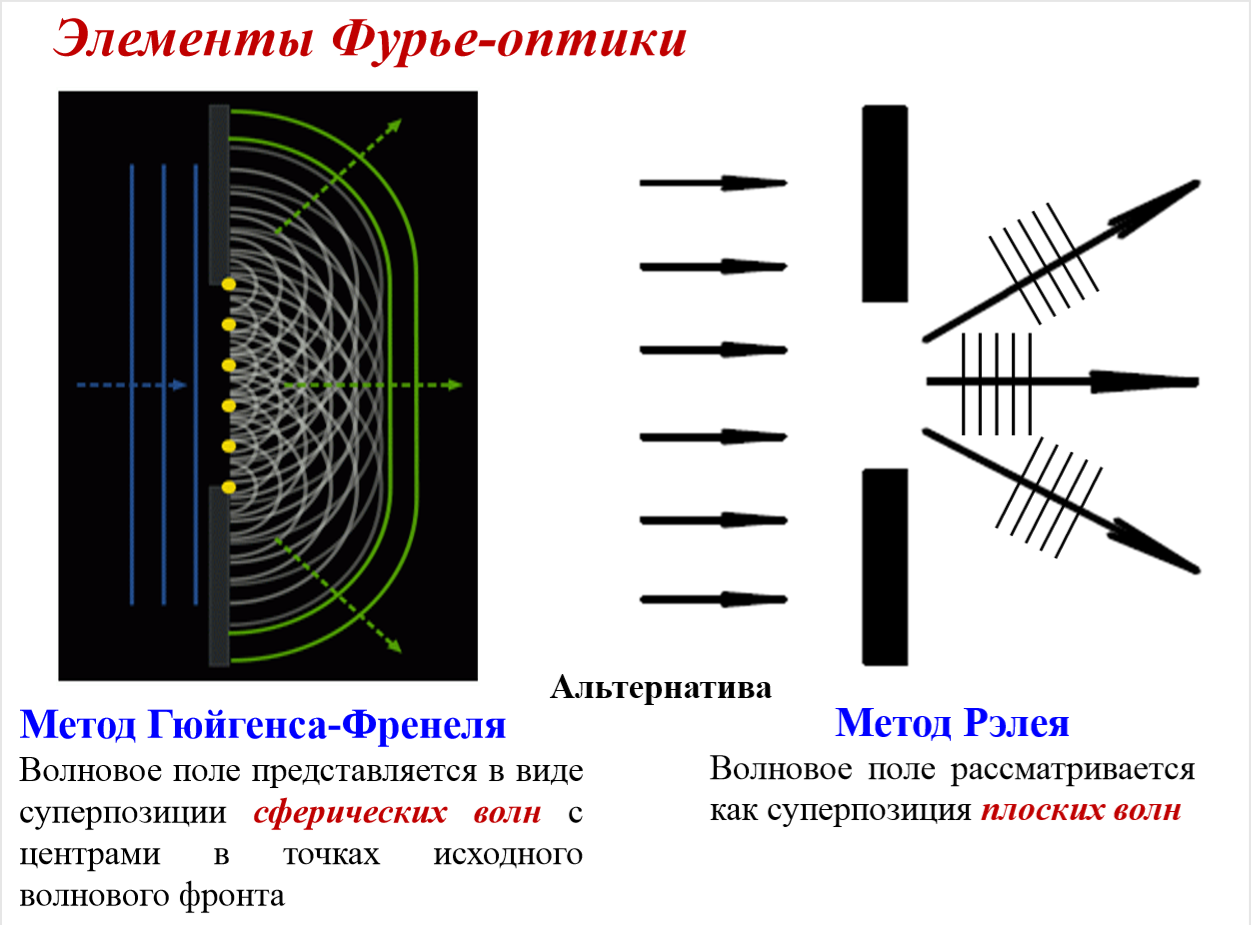
\includegraphics[scale = 0.7]{Rayleigh.png}
    \caption{Иллюстрация лектора}
    \label{fig:my_label}
\end{figure}

\subsection{Явление саморепродукции (эффект Талбота)} Представим себе бесконечный экран, относительно которого введем координаты так, как показано на рисунке (\ref{screen})
\begin{figure}[h]
    \centering
    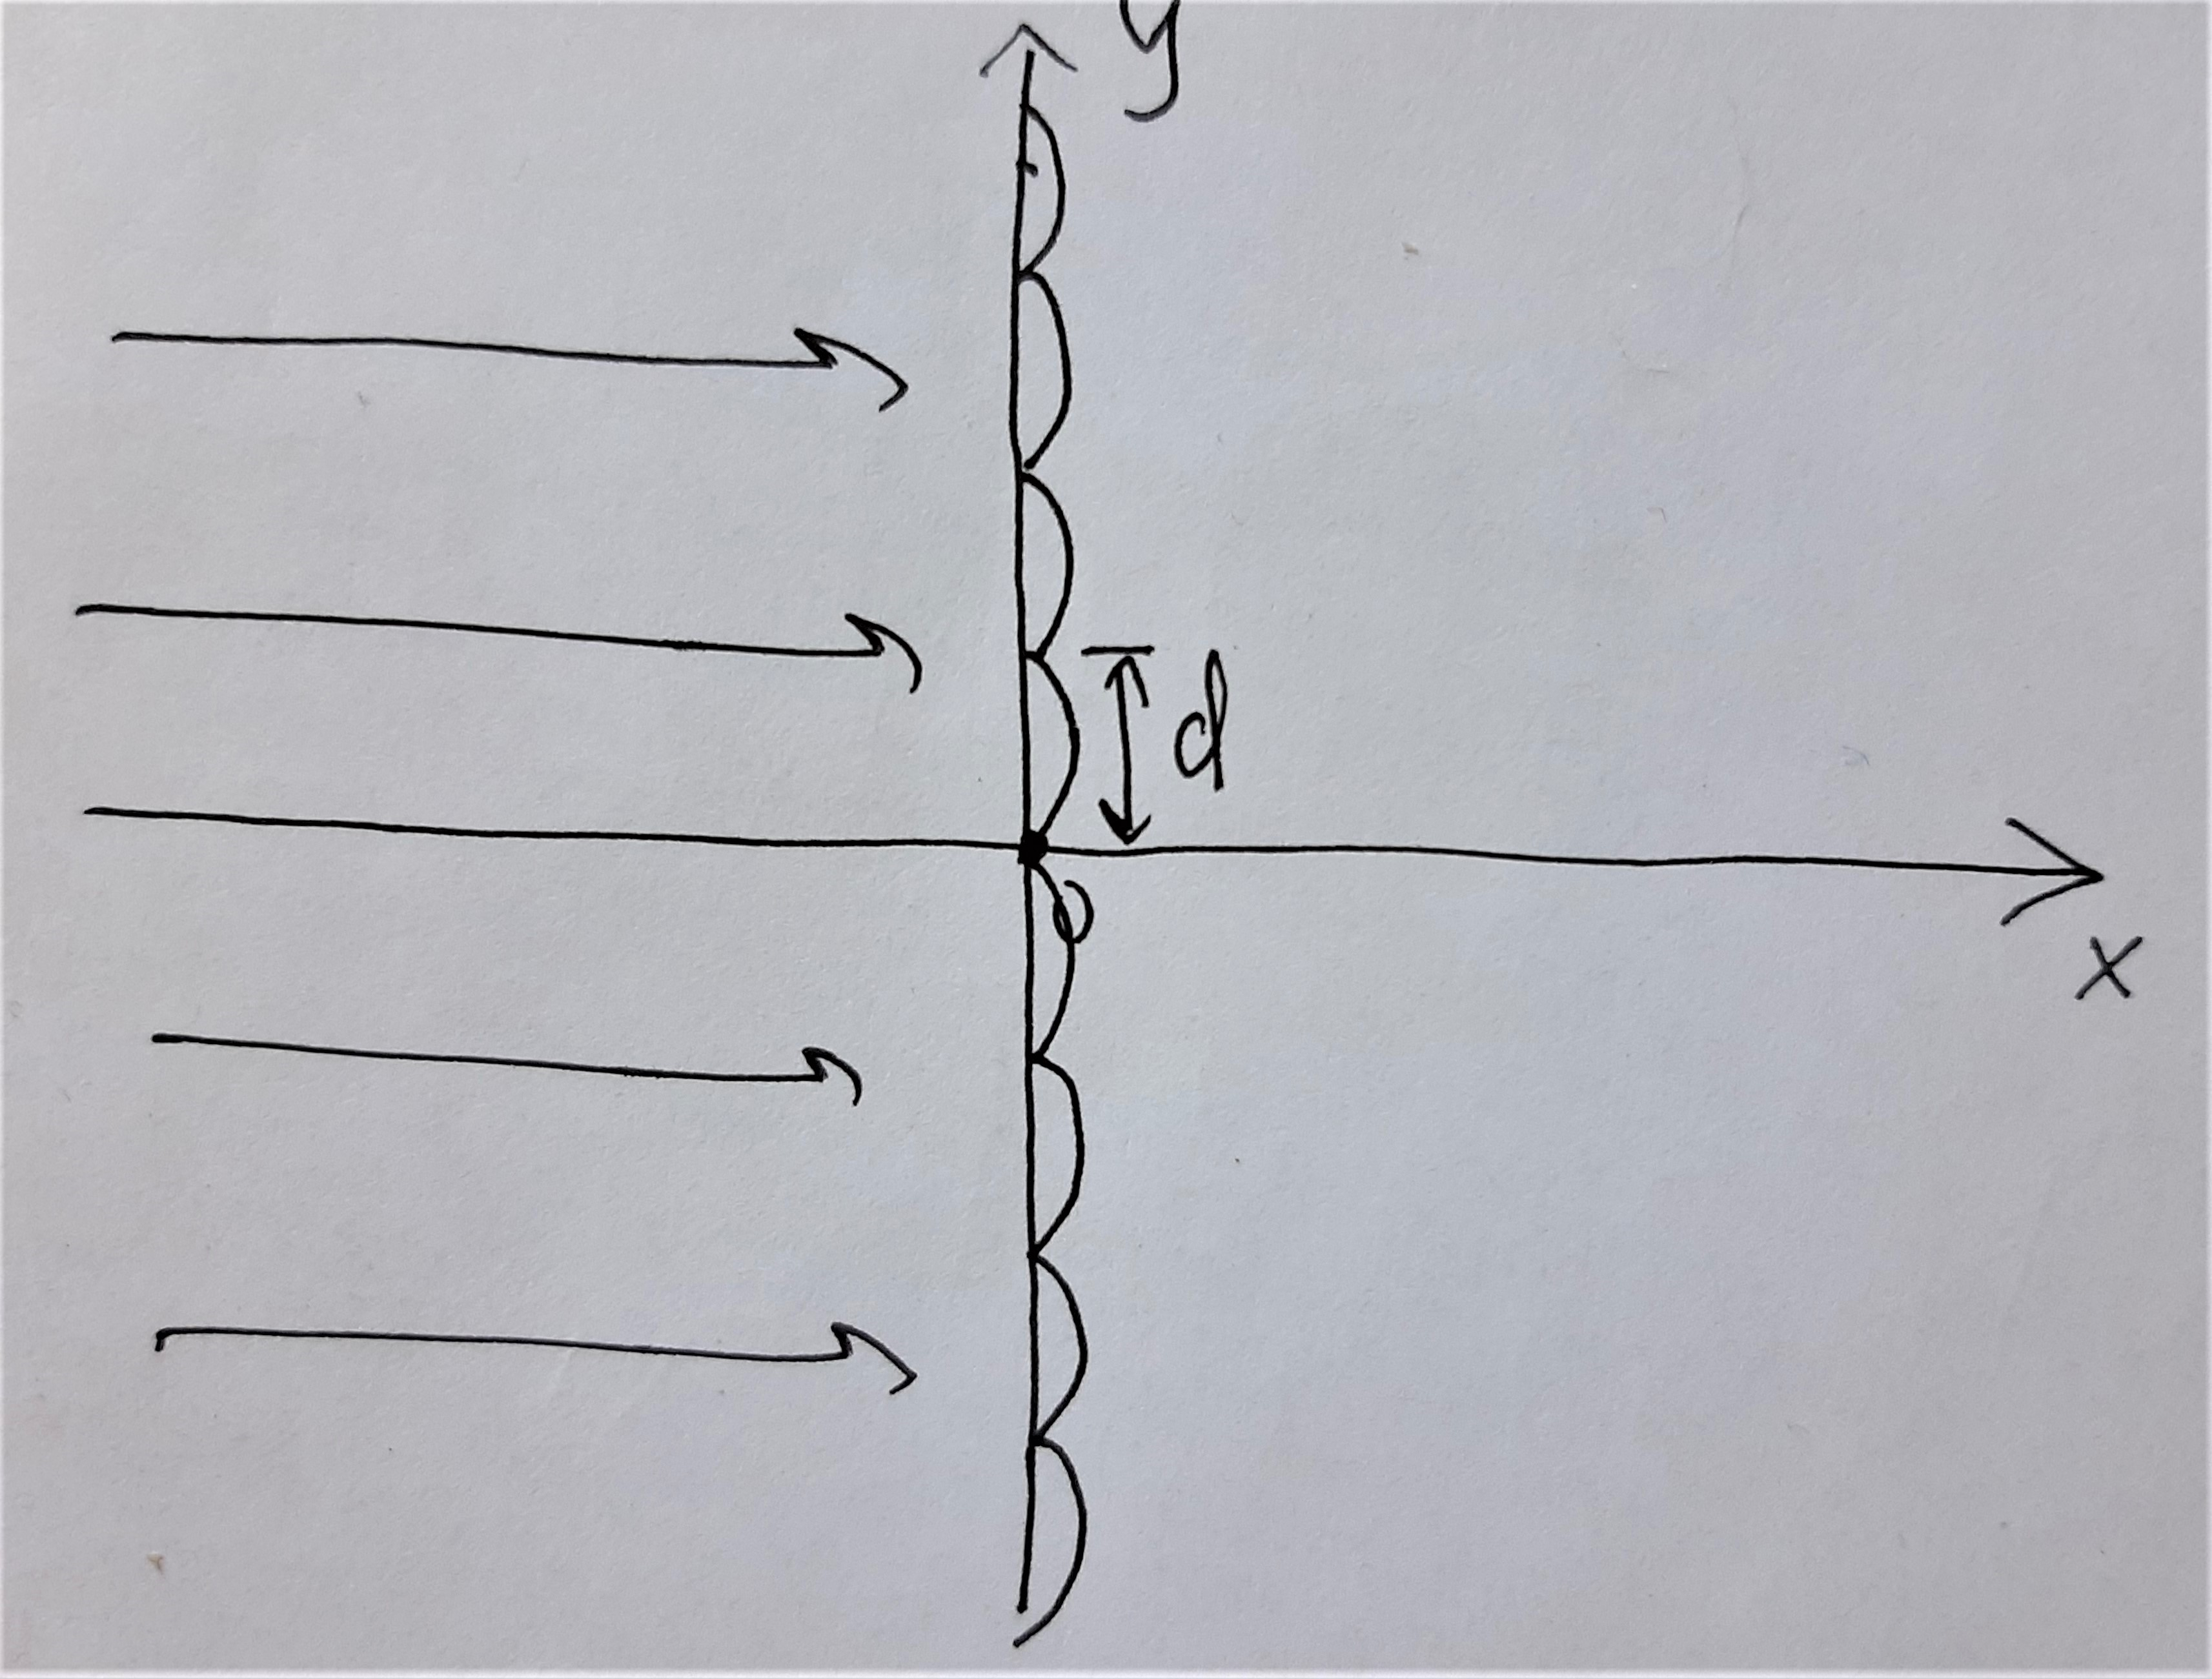
\includegraphics[scale = 0.05]{screen.jpg}
    \caption{Экран с какой-то периодической структурой (это не синусоида) и падающая плоская волна}
    \label{screen}
\end{figure}
Пусть отверстия на экране имеют какую-либо периодическую структуру с пространственным периодом \(d\). Слева на экран перпендикулярно падает плоская волна с волновым вектором \(k\). Тогда справа от экрана мы получим электрическое поле \(E(t = 0, x = 0+)\) в виде периодической функции с периодом, равным периоду решетки \(d\).  Раз поле \(E(t = 0, x = 0+)\) периодическое, мы можем разложить его в ряд Фурье (разложить по плоским волнам, т.е. перейти к представлению Рэлея):
\begin{equation}
    E(t = 0, x = 0+) = \frac{1}{2\pi} \sum_{-\infty}^{\infty} C_n \exp^{in\Omega y}
\end{equation}
\begin{equation}
\Omega = \frac{2\pi}{d}
\end{equation}
В случае, если период решетки больше длины падающей волны, найдется плоская волна, распространяющаяся под таким направлением \(\theta\) к оси \(Ox\), что:
\begin{equation}
\Omega = k sin(\theta)
\end{equation}
То есть, ее пространственная частота по оси \(y\) совпадает с частотой периодической структуры экрана (см. рис. \ref{period}.


\begin{figure}[H]
    \centering
    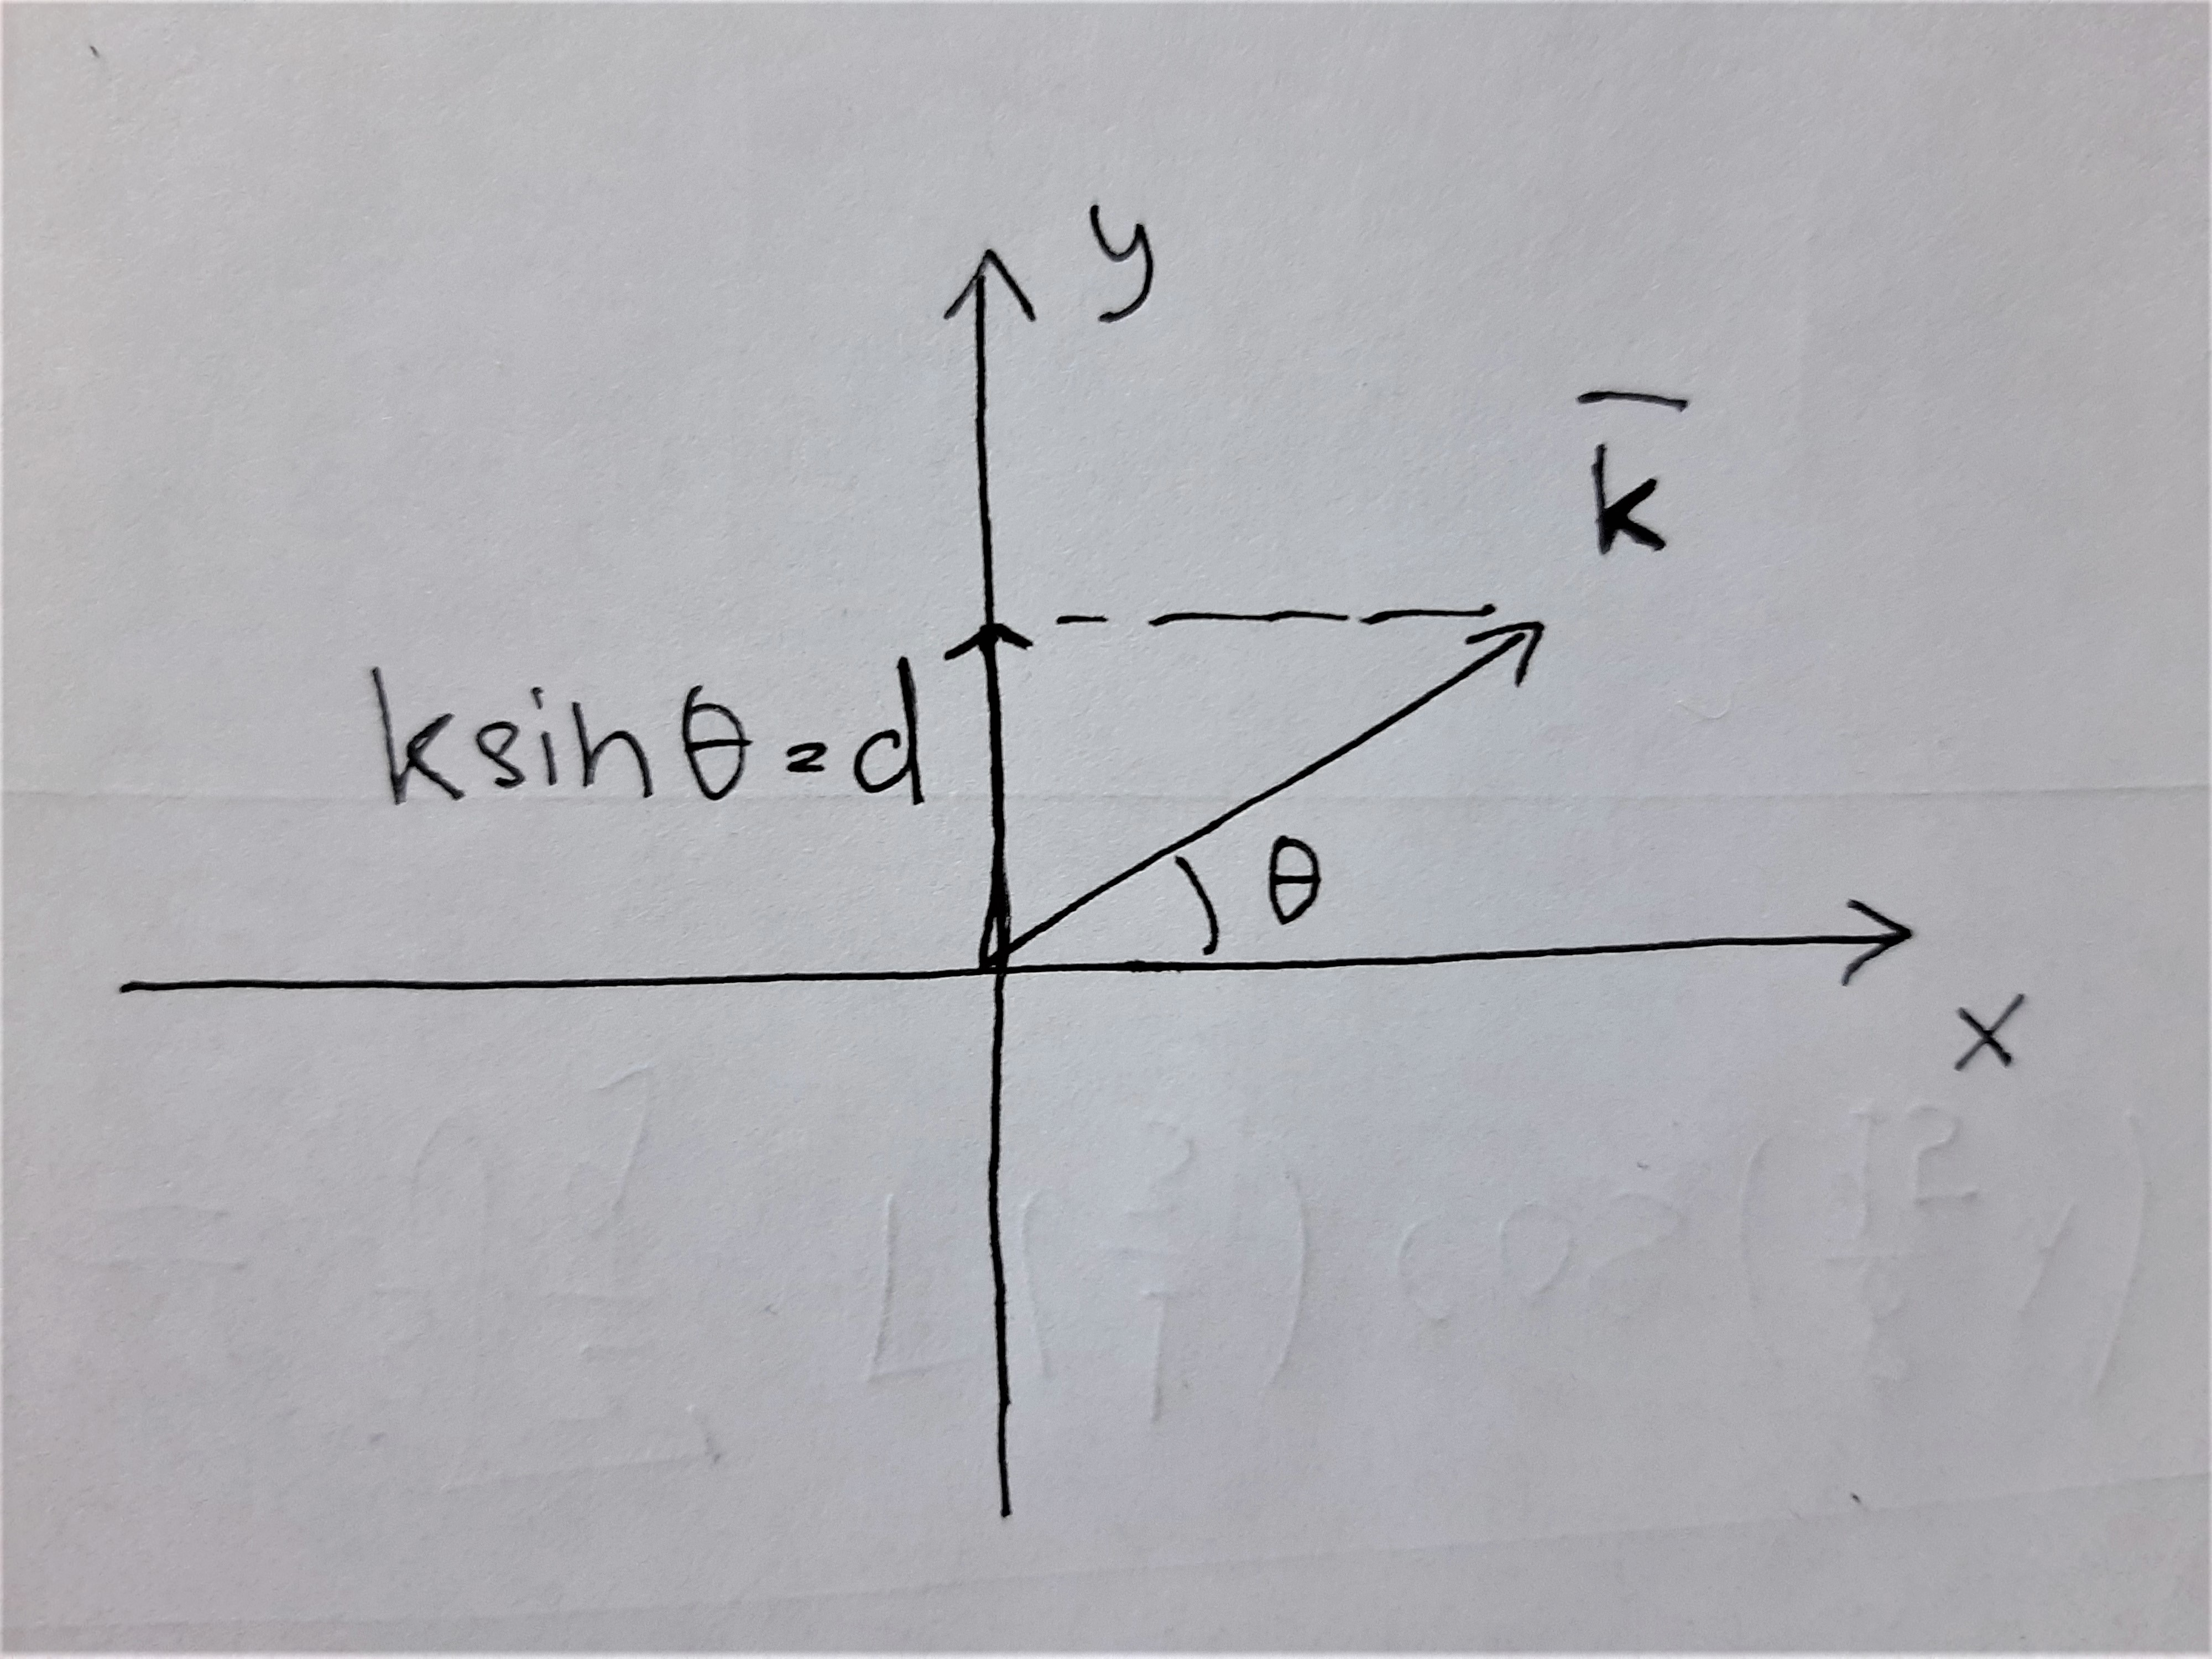
\includegraphics[scale = 0.05]{period.jpg}
    \caption{Выбранная плоская волна}
    \label{period}
\end{figure}


Теперь мы хотим устроить так, чтобы  на расстоянии \(x\) от экрана рассмотренное поле \(E\) \textbf{саморепродуцировалось}. Найдем это расстояние. Выберем произвольную координату по оси \(Oy\) и потребуем, чтобы в ней поле перешло в себя. В терминах представления Рэлея это означает (см. рис. \ref{repro}), что на расстоянии \(x\) от экрана набег фазы между волнами \(e_4\) и \(e_3\) должен быть равен сдвигу фаз между волнами \(e_1, e_0\) с точностью до \(2\pi\).


\begin{figure}[h]
    \centering
    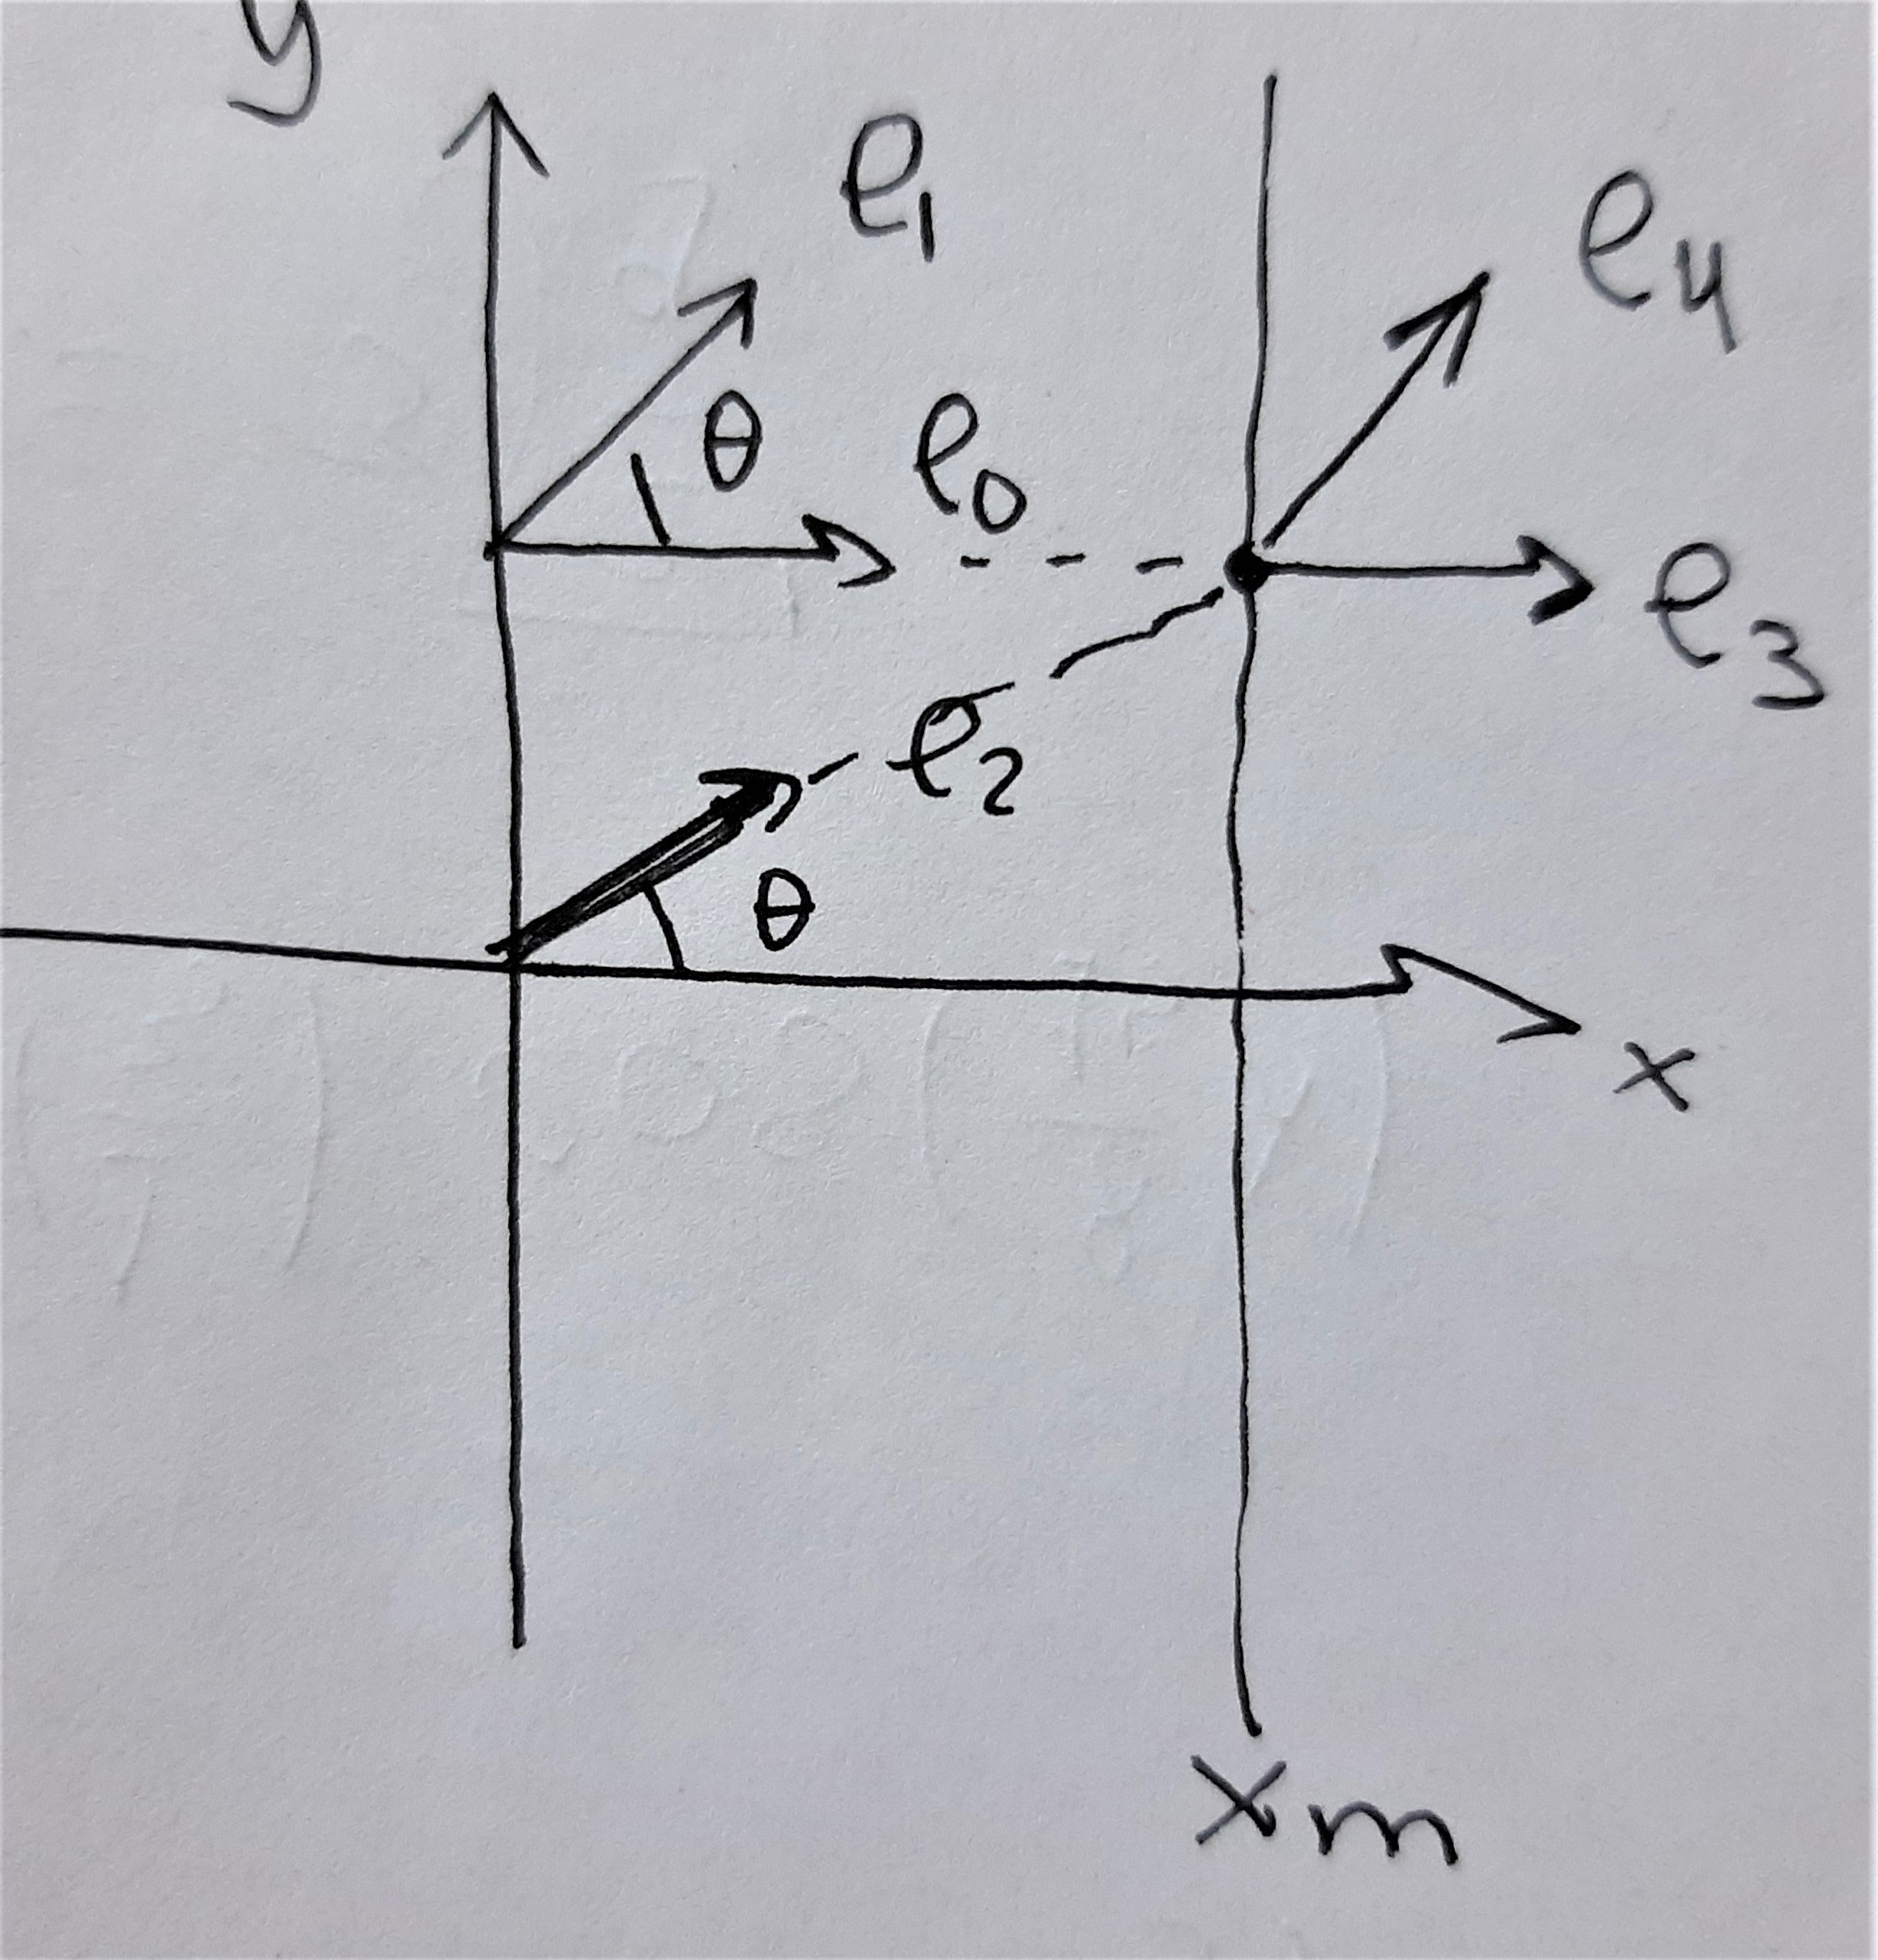
\includegraphics[scale = 0.05]{repro.jpg}
    \caption{Репродукция поля в терминах представления Рэлея}
    \label{repro}
\end{figure}


При этом в волну \(e_4\) переходит волна \(e_2\). Запишем разность набега фаз и найдем \(x_m\):
\begin{equation}
    \omega t - ky\sin(\theta) - kx_m \cos{\theta} - (\omega t - k x_m) = -ky\sin(\theta) + 2 \pi m
\end{equation}
\begin{equation}
     - kx_m \cos(\theta) + k x_m = 2 \pi m
\end{equation}
\begin{equation}
     - kx_m \sqrt{1 - \sin(\theta)^2} + k x_m = 2 \pi m
\end{equation}
В приближении \(\sin(\theta) = \frac{\Omega}{k} = \frac{\lambda}{d} << 1\):
\begin{equation}
     - kx_m (1 - \frac{\lambda^2}{2d^2}) + k x_m = 2 \pi m
\end{equation}
\begin{equation}
    kx_m\frac{\lambda^2}{2d^2} = 2 \pi m
\end{equation}
\begin{equation}
    kx_m \frac{2\pi \lambda}{2 k d^2} = 2 \pi m
\end{equation}
\begin{equation}
    x_m \frac{\lambda}{d^2} = 2 m
\end{equation}

\begin{center}
\fbox{\(x_m = 2 m \frac{d^2}{\lambda}\)}
\end{center}
Красивая картиночка по этому поводу напоследок (рис. \ref{talbot}).
\begin{figure}[H]
    \centering
    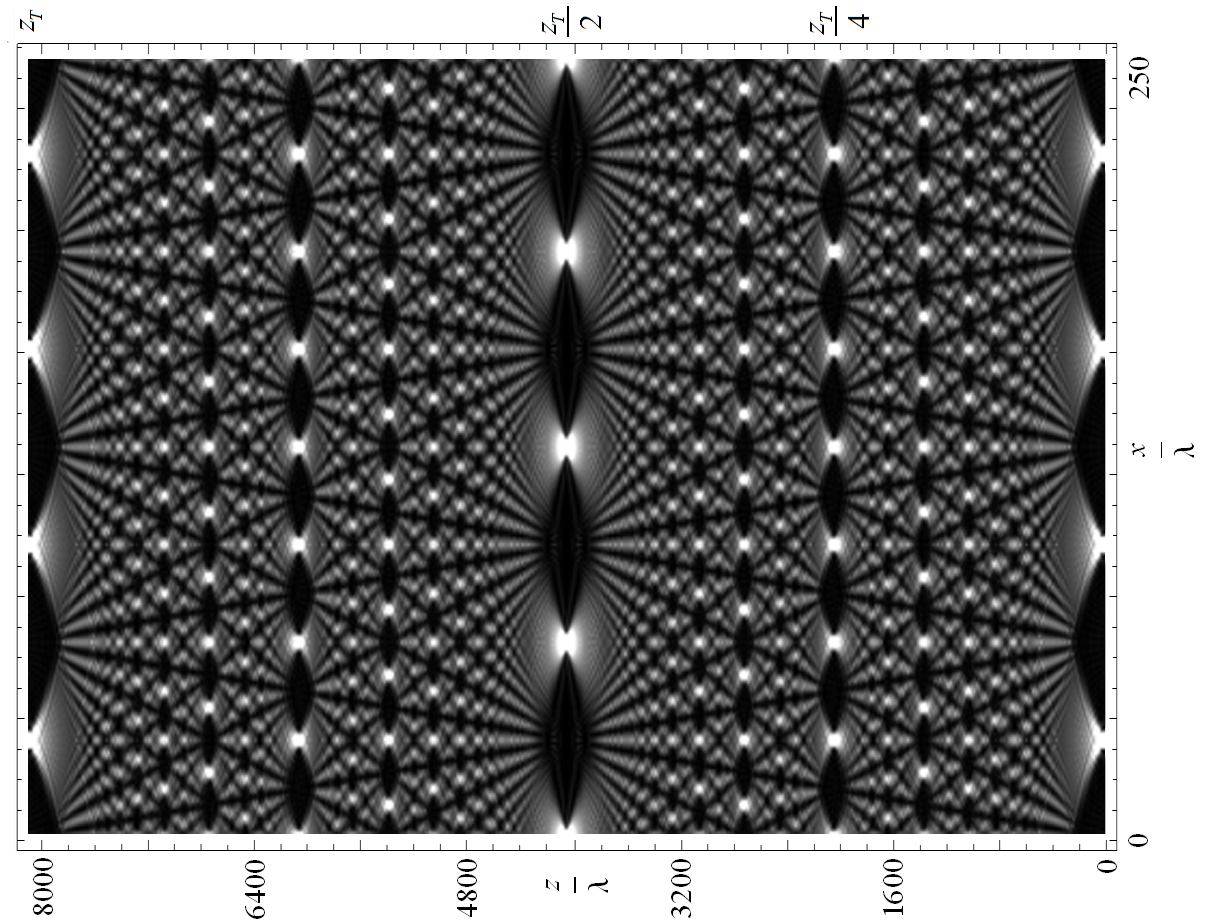
\includegraphics[scale = 0.2]{Optical_Talbot_Carpet.png}
    \caption{Т.н. ковер Талбота}
    \label{talbot}
\end{figure}


Оценка того, сколько раз поле воспроизведет само себя приводится в лекции №15 на слайде 11.


\subsection{Фурье-плоскость}
\textbf{Фурье-плоскость} - фокальная плоскость линзы. Различные плоские волны при прохождении линзы сфокусируются в разные точки в фокальной плоскости. Таким образом, опять получим преобразование Фурье (пространственное).

\subsection{Теория Аббе формирования изображения}
Изображение формируется в два этапа. Свет приходит от предмета на линзу. Линза раскладывает свет по плоским волнам в фокальной плоскости (фурье-плоскости). Получается первичное изображение предмета. Каждая точка в фокальной плоскости является источником вторичных волн. Эти волны интерферируют в плоскости экрана. Получается вторичное изображение предмета.

\subsection{Схема Катрона}
Схема Катрона представлена на рис. \ref{catron}. На месте Ф можно поставить какую-нибудь решетку. Пример от лектора: взять на месте \(P_1\) решетку с периодом \(d\), получить в Ф серию точек, закрыть каждую вторую и получить в \(P_2\) изображение решетки с периодом \(d / 2\).
\begin{figure}[H]
    \centering
    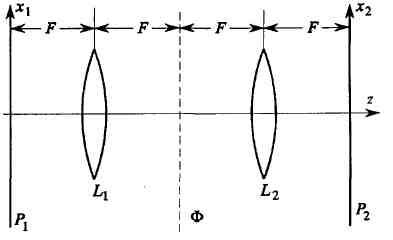
\includegraphics{catron.jpg}
    \caption{Схема Катрона}
    \label{catron}
\end{figure}

\subsection{Методы наблюдения фазовых объектов}
Кириченко, параграф 8.5.1. Вроде все хорошо написано, но нет сил перепечатывать.
